
\section{刻度选项}
\label{sec:pgfplots:ticks}

\subsection{刻度坐标与标签文本}

\begin{pgfplotsxykey}{\x tick distance=\marg{empty or numeric} (initially empty)}
    允许定义生成的刻度\emph{位置}之间的\emph{距离}。

\begin{codeexample}[]
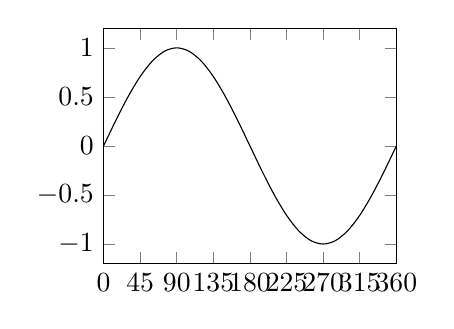
\begin{tikzpicture}
\begin{axis}[
    xtick distance=45,
    ytick distance=0.5,
    enlarge x limits=false,
]
    \addplot [smooth,domain=0:360] {sin(x)};
\end{axis}
\end{tikzpicture}
\end{codeexample}

\begin{codeexample}[]
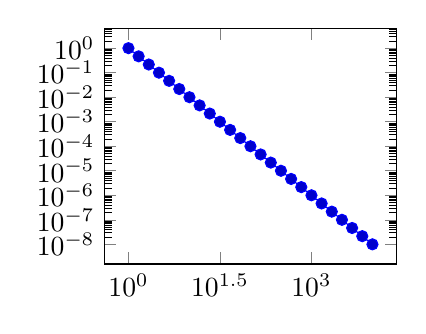
\begin{tikzpicture}
\begin{loglogaxis}[
    xtick distance=10^(1.5),
    ytick distance=10^1,
]
    \addplot expression [domain=1:10000] {x^-2};
\end{loglogaxis}
\end{tikzpicture}
\end{codeexample}

    初始值为空，表示“按需生成”。

    任何其他值都被解释为常量（使用数学表达式解析器求值），并按其原样使用。请注意，此类值的选择应使生成的刻度位置既不太多也不太少。
\end{pgfplotsxykey}

\begin{pgfplotsxykey}{\x tick=\mchoice{%
        \textbackslash empty,
        data,
        \normalfont\marg{coordinate list}%
    } (initially \marg{})%
}
        \index{Tick Labels!Positions: xtick}%
        \index{Tick Labels!Distances: xtick with foreach}%
    这些选项指定一个需要放置刻度的\emph{位置}列表。参数可以是空字符串（即初始值）、命令 |\empty|、特殊字符串 `|data|'，或坐标列表。空字符串的初始配置表示自动生成这些位置。选项 |\empty| 将导致完全没有刻度。特殊值 `|data|' 将在第一个图的每个坐标处产生刻度标记。否则，刻度标记将放置在 \meta{coordinate list} 中的每个坐标处。

    \meta{coordinate list} 将用于 |\foreach \x in |\marg{coordinate list} 语句内部。格式如下：
    %
    \begin{itemize}
        \item |{0,1,2,5,8,1e1,1.5e1}|（一系列坐标），
        \item |{0,...,5}|（与 |{0,1,2,3,4,5}| 相同），
        \item |{0,2,...,10}|（与 |{0,2,4,6,8,10}| 相同），
        \item |{9,...,3.5}|（与 |{9, 8, 7, 6, 5, 4}| 相同），
        \item 有关这些选项更详细的定义，请参阅 \cite[Section~34]{tikz}。
        \item 请注意 \meta{coordinate list} 内部的空白字符（至少在省略号周围）。
    \end{itemize}
    %
    对于对数图，\PGFPlots{} 将对 `\meta{coordinate list}' 中的每个元素应用 $\log(\cdot)$（类似地，任何自定义变换都会应用于参数列表）。
    %
\begin{codeexample}[]
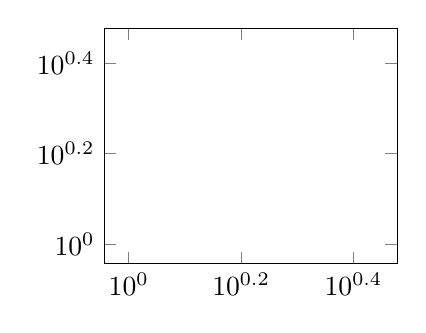
\begin{tikzpicture}
\begin{loglogaxis}[
    xtick={
        12,
        9897,
        1468864
    },
]
    % see above for this macro:
    \plotcoords
\end{loglogaxis}
\end{tikzpicture}
\end{codeexample}

\begin{codeexample}[]
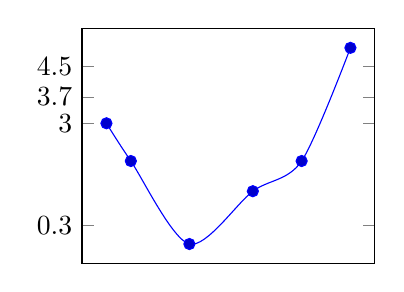
\begin{tikzpicture}
\begin{axis}[
    xtick=\empty,
    ytick={-2,0.3,3,3.7,4.5},
]
    \addplot+ [smooth] coordinates {
        (-2,3) (-1.5,2) (-0.3,-0.2)
        (1,1.2) (2,2) (3,5)
    };
\end{axis}
\end{tikzpicture}
\end{codeexample}

    \paragraph{注意：}

    如果元素对 \TeX{} 来说太大，则不能使用 `|...|' 语法！例如，`|xtick={1.5e5,2e7,3e8}|' 可以工作（因为这些元素被解释为字符串而非数字），但 `|xtick={1.5,3e5,...,1e10}|' 会失败，因为它涉及超出 \TeX{} 能力范围的实数运算。
        \vspace*{0.3cm}

    \noindent 普通图中刻度\emph{位置}的默认选择是在每个坐标~$i\cdot h$ 处放置一个刻度。步长~$h$ 取决于坐标轴缩放和坐标轴界限。它从“可行”步长列表中选择，使生成的刻度既不太多也不太少。对数图的默认做法是在坐标轴范围内的位置 $10^i$ 处放置刻度。这些位置取决于坐标轴缩放和图片尺寸。如果对数图的界限内只包含一个（或两个）位置 $10^i$，则刻度将放置在位置 $10^{i\cdot h}$ 处，并使用与线性坐标轴情况相同的“可行”步长 $h$。

    \noindent 刻度\emph{外观}可以通过以下方式（重新）配置：
    %
\begin{codeexample}[code only]
\pgfplotsset{tick style={very thin,gray}}   % modifies the style `every tick'
\pgfplotsset{minor tick style={black}}      % modifies the style `every minor tick'
\end{codeexample}

    这些样式命令可以随时使用。刻度线宽度可以通过 `|major tick length|' 和 `|minor tick length|' 配置。
    %
\begin{codeexample}[]
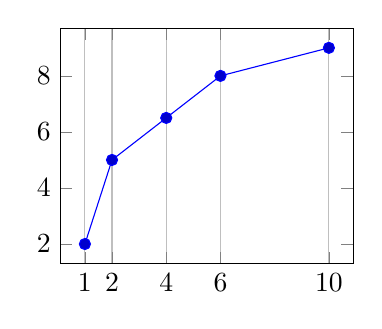
\begin{tikzpicture}
\begin{axis}[
    xtick=data,
    xmajorgrids,
]
    \addplot coordinates {
        (1,2)
        (2,5)
        (4,6.5)
        (6,8)
        (10,9)
    };
\end{axis}
\end{tikzpicture}
\end{codeexample}

\begin{codeexample}[]
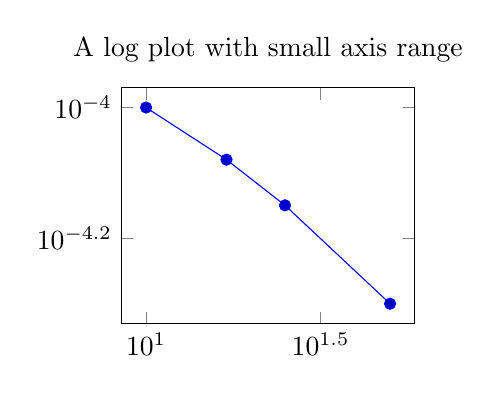
\begin{tikzpicture}
\begin{loglogaxis}[
    title=A log plot with small axis range,
]
    \addplot coordinates {
        (10,1e-4)
        (17,8.3176e-05)
        (25,7.0794e-05)
        (50,5e-5)
    };
\end{loglogaxis}
\end{tikzpicture}
\end{codeexample}
\end{pgfplotsxykey}

\begin{pgfplotsxykeylist}{%
    minor \x\ tick num=\marg{number} (initially 0),
    minor tick num=\marg{number}%
}
    设置用于单个坐标轴或所有坐标轴的次刻度线数量。

    如果主刻度间距不相同，次刻度将被禁用；而且它们目前仅适用于线性坐标轴（不适用于对数坐标轴）。
    %
\begin{codeexample}[]
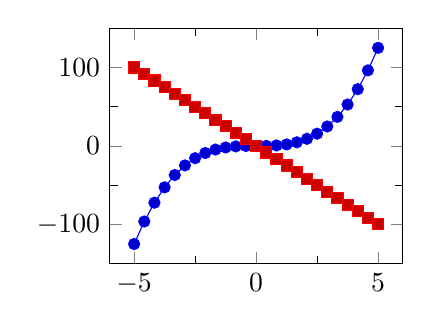
\begin{tikzpicture}
\begin{axis}[
    minor tick num=1,
]
    \addplot {x^3};
    \addplot {-20*x};
\end{axis}
\end{tikzpicture}
\end{codeexample}

\begin{codeexample}[]
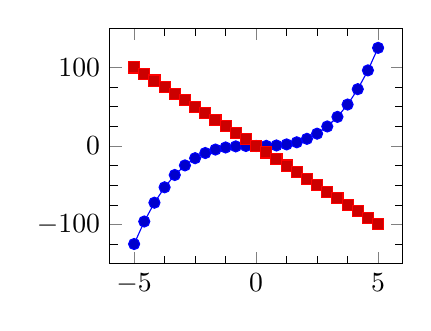
\begin{tikzpicture}
\begin{axis}[
    minor tick num=3,
]
    \addplot {x^3};
    \addplot {-20*x};
\end{axis}
\end{tikzpicture}
\end{codeexample}

\begin{codeexample}[]
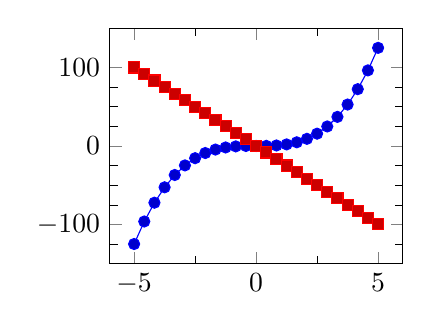
\begin{tikzpicture}
\begin{axis}[
    minor x tick num=1,
    minor y tick num=3,
]
    \addplot {x^3};
    \addplot {-20*x};
\end{axis}
\end{tikzpicture}
\end{codeexample}
\end{pgfplotsxykeylist}

\begin{pgfplotsxykeylist}{%
    minor \x tick=\mchoice{data,\normalfont\marg{coordinate list}} (initially empty),%
    minor tick=\mchoice{data,\normalfont\marg{coordinate list}}%
}
    允许手动提供次刻度位置列表。语法与 |xtick| 或 |ytick| 几乎相同：只需提供逗号分隔的刻度位置列表，或特殊值 |data|。空参数会禁用 |minor tick| 功能（与 |xtick| 不同，在 |xtick| 中特殊值 |\empty| 会清除列表，而空参数会使 \PGFPlots{} 计算默认刻度列表）。

    与 |minor x tick num| 不同，此键允许提供\emph{非均匀}的次刻度位置。
    %
\begin{codeexample}[]
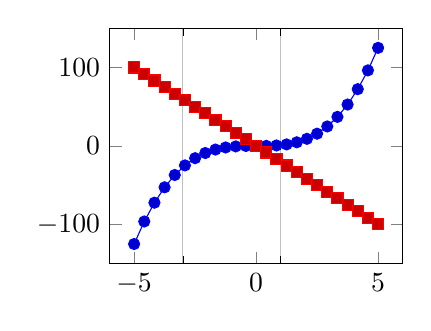
\begin{tikzpicture}
\begin{axis}[
    minor xtick={-3,1},
    grid=minor,
]
    \addplot {x^3};
    \addplot {-20*x};
\end{axis}
\end{tikzpicture}
\end{codeexample}

\begin{codeexample}[]
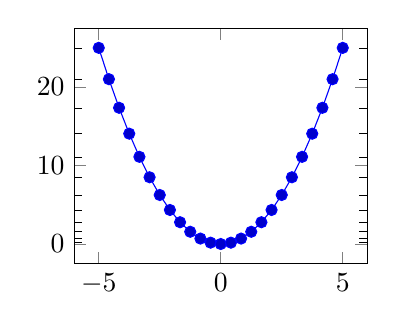
\begin{tikzpicture}
\begin{axis}[
    minor ytick=data,
]
    \addplot {x^2};
\end{axis}
\end{tikzpicture}
\end{codeexample}

    此键优先于 |minor x tick num| 及其变体；如果两者都给出，则优先使用 |minor xtick|，而忽略 |minor x tick num|。
\end{pgfplotsxykeylist}

\begin{pgfplotsxykey}{extra \x\ ticks=\marg{coordinate list}}
    向 $x$ 或 $y$ 坐标轴添加\emph{额外的}刻度位置和刻度标签。“额外的”刻度位置不影响正常的刻度放置算法，它们在正常刻度之后绘制。这有两个好处：第一，你可以添加单个重要的刻度位置而无需禁用默认刻度标签生成；第二，你可以将刻度标签绘制在其他标签“之上”，并可能使用不同的样式标志。
    %
\begin{codeexample}[]
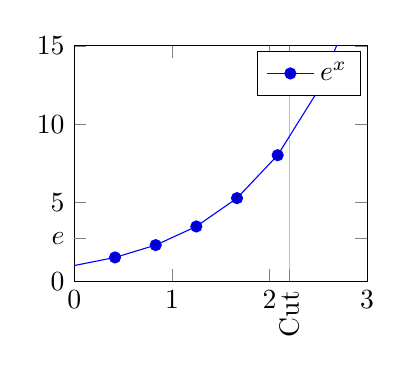
\begin{tikzpicture}
\begin{axis}[
    xmin=0,xmax=3,ymin=0,ymax=15,
    extra y ticks={2.71828},
    extra y tick labels={$e$},
    extra x ticks={2.2},
    extra x tick style={grid=major,
        tick label style={
            rotate=90,anchor=east}},
    extra x tick labels={Cut},
]
    \addplot {exp(x)};
    \addlegendentry{$e^x$}
\end{axis}
\end{tikzpicture}
\end{codeexample}

\message{Overfull hbox is ok.}%
\begin{codeexample}[]
\pgfplotsset{every axis/.append style={width=5.3cm}}
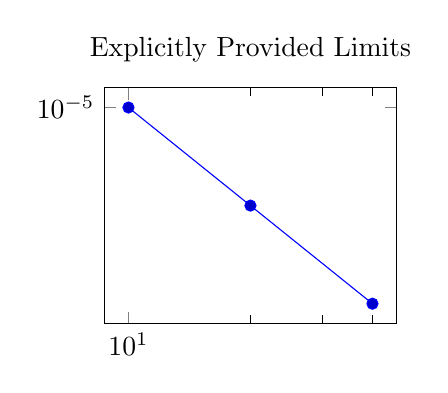
\begin{tikzpicture}
    \begin{loglogaxis}[
        title=Explicitly Provided Limits,
        xtickten={1,2},
        ytickten={-5,-6},
    ]
        \addplot coordinates
            {(10,1e-5) (20,5e-6) (40,2.5e-6)};
    \end{loglogaxis}
\end{tikzpicture}

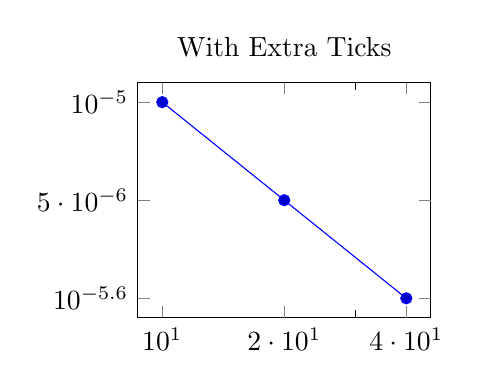
\begin{tikzpicture}
    \begin{loglogaxis}[
        title=With Extra Ticks,
        xtickten={1,2},
        ytickten={-5,-6},
        extra x ticks={20,40},
        extra y ticks={5e-6,2.5e-6},
    ]
        \addplot coordinates
            {(10,1e-5) (20,5e-6) (40,2.5e-6)};
    \end{loglogaxis}
\end{tikzpicture}

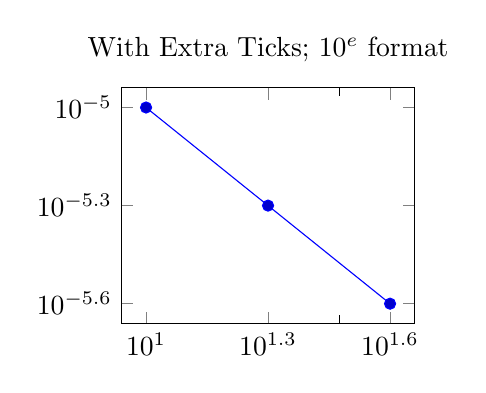
\begin{tikzpicture}
    \begin{loglogaxis}[
        title=With Extra Ticks; $10^e$ format,
        extra tick style={log identify minor tick positions=false},
        xtickten={1,2},
        ytickten={-5,-6},
        extra x ticks={20,40},
        extra y ticks={5e-6,2.5e-6},
    ]
        \addplot coordinates
            {(10,1e-5) (20,5e-6) (40,2.5e-6)};
    \end{loglogaxis}
\end{tikzpicture}
\end{codeexample}

    备注：
    %
    \begin{itemize}
        \item 使用 |extra x ticks| 来突出特殊刻度位置。|extra x ticks| 的使用不影响次刻度/网格线的生成，因此你可以在对数图中将额外刻度放置在位置 $j\cdot 10^i$ 处。
        \item 额外刻度总是被排版为主刻度。

            它们受 |major tick length| 或类似 |grid=major| 的选项影响。
        \item 使用样式 |every extra x tick|（|every extra y tick|）来配置外观。
        \item 你也可以使用 `|extra x tick style=|\marg{...}'，它具有相同的效果。
    \end{itemize}
\end{pgfplotsxykey}

\begin{pgfplotsxykey}{\x tickten=\marg{exponent base 10 list}}
        \index{Tick Labels!Placement of log tick labels: xtickten}%
    这些选项允许在选定的位置 $10^k$（$k \in \text{\marg{exponent base 10 list}}$）处放置刻度。它们仅用于对数图。\marg{exponent base 10 list} 的语法与上面 |xtick=|\marg{list} 或 |ytick=|\marg{list} 的语法相同。

    使用 `|xtickten={1,2,3,4}|' 等价于 `|xtick={1e1,1e2,1e3,1e4}|'，但它需要更少的计算时间，并且允许使用简短语法 `|xtickten={1,...,4}|'。
    %
\begin{codeexample}[]
\begin{tikzpicture}
\begin{semilogyaxis}[
    samples=8,
    ytickten={-6,-4,...,4},
    domain=0:10,
]
    \addplot {2^(-2*x + 6)};
    \addlegendentry{$2^{-2x + 6}$}

    % or invoke gnuplot to generate coordinates:
    \addplot gnuplot [id=pow2]
        {2**(-1.5*x -3)};
    \addlegendentry{$2^{-1.5x -3}$}
\end{semilogyaxis}
\end{tikzpicture}
\end{codeexample}

    如果 |log basis x|$\,\neq 10$，则 |xtickten| 的含义会改变。在这种情况下，|xtickten| 仍将指定指数，但使用所选的 |log basis x| 而非底数 $10$。
\end{pgfplotsxykey}

\begin{pgfplotsxykey}{\x ticklabels=\marg{label list}}
\labelprefix\label{pgfplots:key:xticklabels}%
\index{Tick Labels!Texts as list: xticklabels}%
    为每个刻度位置指定一个刻度\emph{标签}\emph{列表}。刻度\emph{位置}使用 |xtick| 和 |ytick| 选项指定。

    这是直接指定刻度标签的两个选项之一。另一个选项是 |xticklabel=|\marg{command}（或 |yticklabel=|\marg{command}）。选项 `|xticklabel|' 提供更高的灵活性，而 `|xticklabels|' 更易于使用。另请参阅变体 |xticklabels from table|。

    参数 \meta{label list} 具有与刻度相同的格式，即
    %
\begin{codeexample}[code only]
xticklabels={$\frac{1}{2}$,$e$}
\end{codeexample}
    %
    表示双元素列表 $\{\frac 12, e\}$。列表索引与刻度位置的索引对应。如果需要在列表元素内部使用逗号，请使用
    %
\begin{codeexample}[code only]
xticklabels={{0,5}, $e$}.
\end{codeexample}

\begin{codeexample}[]
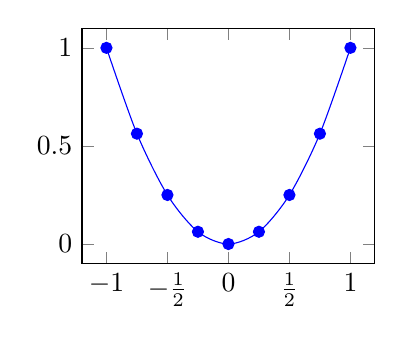
\begin{tikzpicture}
\begin{axis}[
    xtick={-1.5,-1,...,1.5},
    xticklabels={%
        $-1\frac 12$,
        $-1$,
        $-\frac 12$,
        $0$,
        $\frac 12$,
        $1$},
    % note: \frac can be done automatically:
    % xticklabel style={/pgf/number format/frac},
]
    \addplot [smooth,blue,mark=*] coordinates {
        (-1,    1)
        (-0.75, 0.5625)
        (-0.5,  0.25)
        (-0.25, 0.0625)
        (0,     0)
        (0.25,  0.0625)
        (0.5,   0.25)
        (0.75,  0.5625)
        (1,     1)
    };
\end{axis}
\end{tikzpicture}
\end{codeexample}

\begin{codeexample}[]
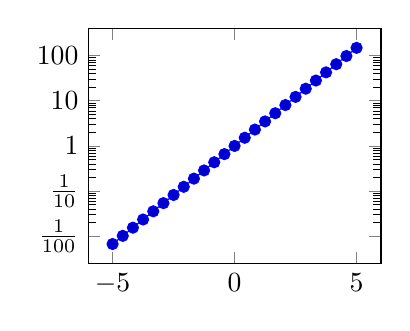
\begin{tikzpicture}
\begin{semilogyaxis}[
    ytickten={-2,-1,0,1,2},
    yticklabels={
        $\frac{1}{100}$,
        $\frac{1}{10}$,
        1,10,100
    },
]
    \addplot {exp(x)};
\end{semilogyaxis}
\end{tikzpicture}
\end{codeexample}

    请注意，也可以用两个反斜杠 |\\| 来结束列表条目。在这种情况下，最后一个条目也需要用 |\\| 结束（这是同样的替代语法，也被 |\legend| 和 |cycle list| 接受）。

    请记住，这些参数\emph{始终}引用刻度位置列表，尽管它并不更改或定义位置列表。因此，你也应该提供位置列表。请注意，位置列表可能比实际显示的更长（在坐标轴界限裁剪掉某些值的情况下），但到 \meta{label list} 的索引映射仍包含被裁剪的值。
\end{pgfplotsxykey}


\begin{pgfplotsxykey}{\x ticklabel=\marg{command}}
        \index{Tick Labels!Configure texts by command: xticklabel}%
    这些键更改用于创建分配给每个刻度位置的刻度\emph{标签}的 \TeX{} 命令（参见选项 |xtick| 和 |ytick|）。

    这是直接指定刻度标签的两个选项之一。另一个选项是 `|xticklabels=|\marg{label list}'（或 |yticklabels=|\marg{label list}）。选项 `|xticklabel|' 提供更高的灵活性，而 `|xticklabels|' 更易于使用。

    参数 \meta{command} 可以是任何 \TeX{} 文本。以下命令在 \meta{command} 内部有效：
    %
    \begin{description}
        \item[] \declareandlabel{\tick} 选项 |xtick|（或 |ytick|）的当前元素。
        \item[] \declareandlabel{\ticknum} 当前刻度编号，从~0 开始（它是一个包含数字的宏）。
        \item[] \declareandlabel{\nexttick} 此命令仅在设置了 |x tick label as interval| 选项（或~$y$ 的相应变量）时有效。它将包含下一个刻度位置的位置，即刻度区间的右边界。
    \end{description}
    %
    默认参数为
    %
    \begin{itemize}
        \item 普通图的 \declareandlabel{\axisdefaultticklabel}：
            %
\begin{codeexample}[code only]
\def\axisdefaultticklabel{$\pgfmathprintnumber{\tick}$}
\end{codeexample}
            %
        \item 对数图的 \declareandlabel{\axisdefaultticklabellog}：
\begin{codeexample}[code only]
\def\axisdefaultticklabellog{%
    \pgfkeysgetvalue{/pgfplots/log number format code/.@cmd}\pgfplots@log@label@style
    \expandafter\pgfplots@log@label@style\tick\pgfeov
}
\end{codeexample}
    \end{itemize}
    %
    这意味着你可以使用 Section~\ref{sec:number:printing} 中描述的数字格式化选项来配置线性坐标轴的外观，使用 |log number format code| 配置对数坐标轴的外观，见下文。

    \noindent 键 |yticklabel| 是一个代码片段，用于处理任何传入的 |\tick| 值。因此，它可用于附加自定义后缀甚至单位：
    %
\begin{codeexample}[]
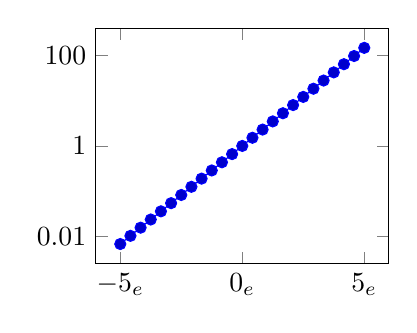
\begin{tikzpicture}
\begin{semilogyaxis}[
    log ticks with fixed point,
    xticklabel={$\pgfmathprintnumber{\tick}_e$},
]
    \addplot {exp(x)};
\end{semilogyaxis}
\end{tikzpicture}
\end{codeexample}

    下面的示例使用显式格式化的 $x$ 刻度标签和一段小型 \TeX{} 脚本，将 $y$ 刻度标签格式化为 \meta{sign}\meta{number}|/10| 形式的分数（请注意，|/pgf/number format/frac| 样式可以自动完成类似的事情，参见 \PGFPlotstable{} 及其中的文档）。
    %
% \usepackage{nicefrac}
\begin{codeexample}[width=4cm]
% \usepackage{nicefrace}% required
\begin{tikzpicture}
    \begin{axis}[
        % x ticks explicitly formatted:
        xtick={0,1,0.5,0.25,0.75},
        xticklabels={$0$,$1$,$\frac12$,$\frac14$,$\frac34$},
        % y ticks automatically by some code fragment:
        ytick=data,
        yticklabel={
            \scriptsize
            \ifdim\tick pt<0pt % a TeX \if -- see TeX Book
                \pgfmathparse{-10*\tick}
                $-\nicefrac{\pgfmathprintnumber{\pgfmathresult}}{10}$
            \else
                \ifdim\tick pt=0pt
                \else
                    \pgfmathparse{10*\tick}
                    $\nicefrac{\pgfmathprintnumber{\pgfmathresult}}{10}$
                \fi
            \fi
        },
        % NOTE: this here does the same:
        % yticklabel style={/pgf/number format/.cd,frac,
        %     frac TeX=\nicefrac,frac whole=false,frac denom=10},
        ymajorgrids,
        title=A special Prewavelet,
        axis x line=center,
        axis y line=left,
    ]
        \addplot coordinates {(0,-1.2) (0.25,1.1)
            (0.5,-0.6) (0.75,0.1) (1,0)};
    \end{axis}
\end{tikzpicture}
\end{codeexample}
    %
    \noindent 该 \TeX{} 脚本以 |\tick| 宏作为输入并应用一些逻辑。|\ifdim\tick pt<0pt| 表示“如果尺寸 |\tick pt| $<$ |0pt|”。|\ifdim| 是 \TeX{} 比较实数定点数的唯一方式，作者不想为此简单任务调用 |\pgfmath|。由于 |\ifdim| 需要一个尺寸，我们必须使用与 |\pgfmath| 兼容的 |pt| 后缀。结果是负数、零和正数被不同地排版。

    你可以通过以下方式更改刻度标签的外观：
    %
\begin{codeexample}[code only]
\pgfplotsset{
    % this modifies the `every tick label' style
    tick label style={
        font=\tiny,
        /pgf/number format/sci,
    },
}
\end{codeexample}
    %
    和/或
    %
\begin{codeexample}[code only]
\pgfplotsset{
    % this modifies the `every x tick label' style
    x tick label style={
        above,
        /pgf/number format/fixed zerofill,
    },
}
\end{codeexample}
    %
    以及
    %
\begin{codeexample}[code only]
\pgfplotsset{
    % modifies `every y tick label'
    y tick label style={font=\bfseries},
}
\end{codeexample}
\end{pgfplotsxykey}

\begin{pgfplotsxykey}{\x ticklabels from table=\marg{\textbackslash table or filename}\marg{colname}}
       \index{Tick Labels!Read from table}%
    |xticklabels=|\marg{list} 的一个变体，它使用表格中名为 \meta{colname} 的列中的每个条目作为刻度标签。

    第一个参数 \meta{\textbackslash table or filename} 可以是已加载的表格宏（即 |\pgfplotstableread|\marg{file name}\marg{\textbackslash table} 的结果），或者只是一个文件名。

    第二个参数可以是列名、列别名或 |create on use| 规范（后两者参见 \PGFPlotstable{}）。此外，它可以是 |[index]|\meta{integer}，此时 \meta{integer} 是列索引。

    |xticklabels from table| 的行为与将列 \meta{colname} 作为逗号分隔列表提供给 |xticklabels| 相同。这意味着该列可以包含文本、\TeX{} 宏，甚至数学模式。

    如果单元格中包含空白字符，请将整个单元格用花括号括起来，如 |{example cell}|。表格的详细输入格式在 \verbpdfref{\addplot table} 和 \PGFPlotstable{} 的文档中讨论。
\end{pgfplotsxykey}

\begin{pgfplotsxykey}{extra \x\ tick label=\marg{\TeX{} code}}
    正如 |xticklabel| 提供为每个 |xtick| 生成刻度标签的代码一样，键 |extra x tick label| 提供为 |extra x ticks| 中每个元素生成刻度标签的代码。
\end{pgfplotsxykey}

\begin{pgfplotsxykey}{extra \x\ tick labels=\marg{label list}}
    正如 |xticklabels| 为每个 |xtick| 提供显式刻度标签一样，键 |extra x tick labels| 为 |extra x ticks| 中的每个元素提供显式刻度标签。
\end{pgfplotsxykey}

\begin{pgfplotsxykey}{\x\ tick label as interval=\mchoice{true,false} (initially false)}
\labelprefix\label{key:pgfplots:ticklabelasinterval}
    允许将刻度标签视为区间；即刻度位置表示区间边界。如果有 $n$ 个位置，将生成 $(n-1)$ 个刻度标签，每个区间一个。
    %
\begin{codeexample}[]
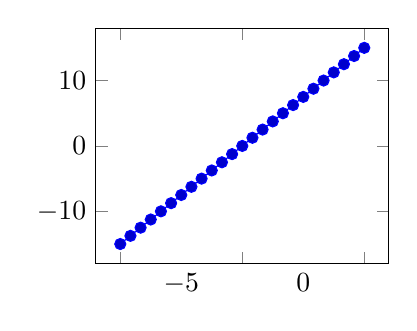
\begin{tikzpicture}
\begin{axis}[
    x tick label as interval,
]
    \addplot {3*x};
\end{axis}
\end{tikzpicture}
\end{codeexample}
    %
    此模式允许在 |xticklabel|（或 |yticklabel|）内部使用 |\nexttick|。一个常见应用可能是条形图。
    %
\begin{codeexample}[]
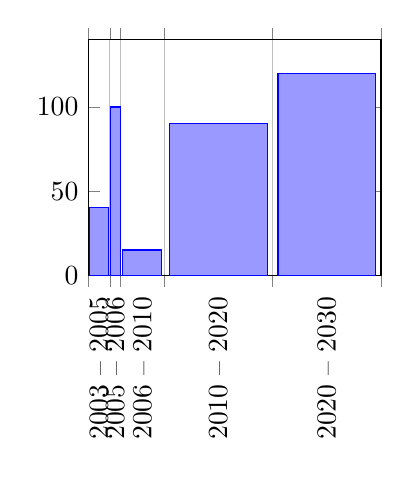
\begin{tikzpicture}
\begin{axis}[
    ybar interval=0.9,
    x tick label as interval,
    xmin=2003,xmax=2030,
    ymin=0,ymax=140,
    xticklabel={
           $\pgfmathprintnumber{\tick}$
        -- $\pgfmathprintnumber{\nexttick}$},
    xtick=data,
    x tick label style={
        rotate=90,anchor=east,
        /pgf/number format/1000 sep=%
    },
]
    \addplot [draw=blue,fill=blue!40!white]
        coordinates
        {(2003,40) (2005,100) (2006,15)
         (2010,90) (2020,120) (2030,3)};
\end{axis}
\end{tikzpicture}
\end{codeexample}
\end{pgfplotsxykey}

\begin{pgfplotsxykeylist}{%
    \x minorticks=\mchoice{true,false} (initially true),
    \x majorticks=\mchoice{true,false} (initially true),
    ticks=\mchoice{minor,major,both,none} (initially both)%
}
    为单个坐标轴或所有坐标轴启用/禁用小刻度线。主刻度是放置在刻度位置处的刻度，次刻度位于刻度位置之间。请注意，如果 |xtick| 不是均匀范围，次刻度会自动禁用。\footnote{均匀列表表示对于线性坐标轴，所有元素之间的差值相同；对于对数坐标轴，则为 $\log(10)$。}

    键 |minor tick length=|\marg{dimen} 配置次刻度的长度，而 |major| 变体适用于主刻度。你可以使用以下样式配置外观：
    %
\begin{codeexample}[code only]
\pgfplotsset{every tick/.append style={color=black}} % applies to major and minor ticks,
\pgfplotsset{every minor tick/.append style={thin}}  % applies only to minor ticks,
\pgfplotsset{every major tick/.append style={thick}} % applies only to major ticks.
\end{codeexample}
    %
    还有一个样式 ``|every tick|''，它同时适用于主刻度和次刻度。
\end{pgfplotsxykeylist}

\begin{pgfplotsxykeylist}{\x tickmin=\marg{coord}, \x tickmax=\marg{coord}}
    这些键可用于在绘制刻度之前修改最小/最大值。由于这适用于坐标轴间断，它在 Section~\ref{sec:axis:discontinuities}（“坐标轴间断”）的第~\pageref{key:xytickminmax} 页中描述。
\end{pgfplotsxykeylist}


\subsection{刻度对齐：位置与偏移}

\begin{pgfplotsxykeylist}{%
    \x tick pos=\mchoice{lower,upper,bottom,top,left,right,both} (initially both),
    tick pos=\mchoice{lower,upper,bottom,top,left,right,both}%
}
    允许选择小刻度线的放置位置。在默认配置下，这也会影响刻度\emph{标签}，见下文。样式 |tick pos| 将它们全部设置为相同的值（由 |tickpos|\pgfmanualpdflabel{/pgfplots/tickpos} 别名）。此选项仅对带框坐标轴有用。

    请注意，键 \declaretext{left} 和 \declaretext{bottom} 是 |lower| 的别名。类似地，\declaretext{right} 和 \declaretext{top} 是 |upper| 的别名。

    更改 |tick pos| 也会影响刻度标签的放置。

    请注意，它也可能影响 |axis lines| 键，尽管并非所有组合都有意义。请确保设置一致。
\end{pgfplotsxykeylist}

\begin{pgfplotsxykeylist}{%
    \x ticklabel pos=\mchoice{lower,upper,bottom,top,left,right,default} (initially default),
       ticklabel pos=\mchoice{lower,upper,bottom,top,left,right,default} (initially default)%
}
    允许选择刻度\emph{标签}的放置位置。选项 |lower| 和 |upper| 将刻度标签放置在整个坐标轴的下侧或上侧。选项 |default| 使用与 |xtick pos|（或 |ytick pos|）相同的设置。此选项仅对带框坐标轴有用——对于非带框图形，请保持为 |default|。样式 |ticklabel pos| 将这三个全部设置为相同的值。

    请注意，键 \declaretext{left} 和 \declaretext{bottom} 是 |lower| 的别名。类似地，\declaretext{right} 和 \declaretext{top} 是 |upper| 的别名。
\end{pgfplotsxykeylist}

\begin{pgfplotsxykeylist}{%
    \x tick align=\mchoice{inside,center,outside} (initially inside),
       tick align=\mchoice{inside,center,outside} (initially inside)%
}
    允许更改刻度相对于坐标轴线的位置。|tick align| 将它们全部设置为相同的值。默认为 ``|inside|''。
    %
\begin{codeexample}[]
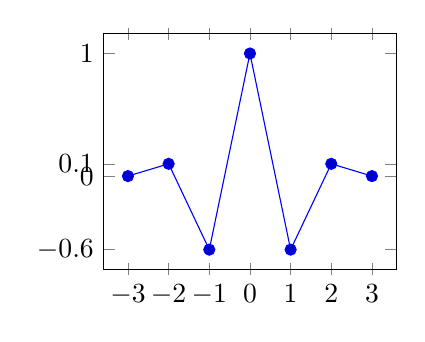
\begin{tikzpicture}
\begin{axis}[
    xtick=data,ytick=data,
    xtick align=center,
]
    \addplot coordinates {
        (-3,0) (-2,0.1) (-1,-0.6)
        (0,1)
        (1,-0.6) (2,0.1) (3,0)
    };
\end{axis}
\end{tikzpicture}
\end{codeexample}

\begin{codeexample}[]
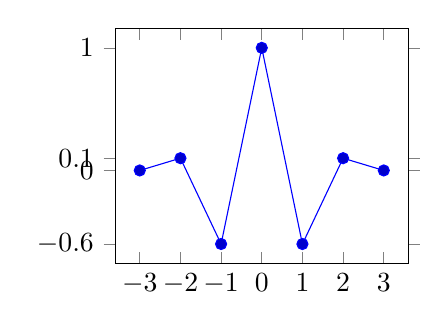
\begin{tikzpicture}
\begin{axis}[
    xtick=data,ytick=data,
    ytick align=outside,
]
    \addplot coordinates {
        (-3,0) (-2,0.1) (-1,-0.6)
        (0,1)
        (1,-0.6) (2,0.1) (3,0)
    };
\end{axis}
\end{tikzpicture}
\end{codeexample}

    这些刻度对齐选项由 |axis x line| 和 |axis y line| 方法自动设置（除非附加了星号 `|*|'）：
    %
\begin{codeexample}[]
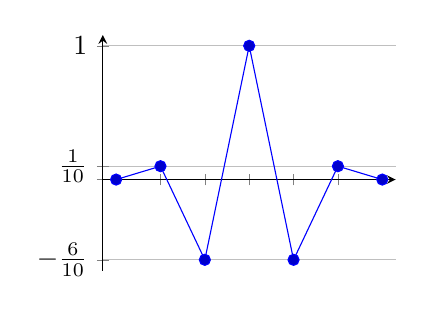
\begin{tikzpicture}
\begin{axis}[
    xtick=data,
    axis x line=center,
    xticklabels={,,},
    ytick={-0.6,0,0.1,1},
    yticklabels={
        $-\frac{6}{10}$,,
        $\frac{1}{10}$,$1$},
    ymajorgrids,
    axis y line=left,
    enlargelimits=0.05
]
    \addplot coordinates {
        (-3,0) (-2,0.1) (-1,-0.6)
        (0,1)
        (1,-0.6) (2,0.1) (3,0)
    };
\end{axis}
\end{tikzpicture}
\end{codeexample}
\end{pgfplotsxykeylist}

\begin{pgfplotsxykeylist}{%
    \x ticklabel shift=\marg{dimension} (initially empty),
       ticklabel shift=\marg{dimension} (initially empty)%
}
       \index{Tick Labels!Shift along normal vector: ticklabel shift}%
    沿坐标轴外单位法线方向将刻度标签偏移 \meta{dimension} 的量。|ticklabel shift| 为所有坐标轴设置相同的值。

    这通常是不必要的，因为在大多数情况下，刻度标签的 |anchor| 已经产生了足够的间距。

    另请参阅 |axis line shift|。
\end{pgfplotsxykeylist}

\begin{pgfplotskeylist}{%
    typeset ticklabels with strut,
    default typeset ticklabel%
}
        \index{Tick Labels!Different Depths}%
        \index{Tick Labels!strut}%
    通常，\PGFPlots{} 按“原样”排版刻度。这几乎在所有情况下都运行良好，尤其是当你只有数字作为刻度标签时。

    但是，如果一个刻度标签在基线下方有文字而另一个没有，则需要调整。|typeset ticklabels with strut| 的目的就是对齐它们。
    %
\begin{codeexample}[]
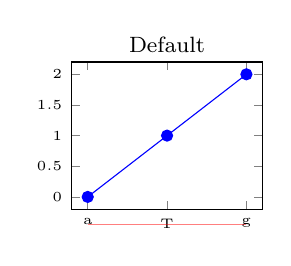
\begin{tikzpicture}
    \begin{axis}[
        title=Default,
        tiny,
        symbolic x coords={a,T,g},
        xticklabel style={name=tick no \ticknum},
        xtick=data,
    ]
        \addplot coordinates {(a,0) (T,1) (g,2)};
    \end{axis}
    \draw [red,opacity=0.5]
        (tick no 0.base) -- (tick no 2.base);
\end{tikzpicture}
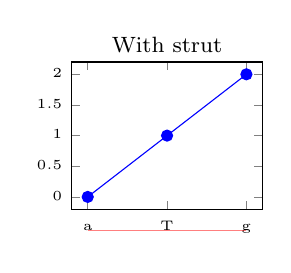
\begin{tikzpicture}
    \begin{axis}[
        title=With strut,
        tiny,
        symbolic x coords={a,T,g},
        xtick=data,
        xticklabel style={name=tick no \ticknum},
        typeset ticklabels with strut,
    ]
        \addplot coordinates {(a,0) (T,1) (g,2)};
    \end{axis}
    \draw [red,opacity=0.5]
        (tick no 0.base) -- (tick no 2.base);
\end{tikzpicture}
\end{codeexample}

    为了规范化刻度标签，\PGFPlots{} 会自动插入 |\strut|。|\strut| 是一个 \TeX{} 宏，它插入一个“全高”的空盒子，包括文本基线上下的所有内容。

    对于标准坐标轴，此键基本等价于 |xticklabel=\strut\pgfmathprintnumber{\tick}|。

    请注意，|\strut| 默认是关闭的，因为它会为纯数字节点不必要地放大包围盒。这对于 |polaraxis| 尤其出乎意料，但对普通图也是如此。
\end{pgfplotskeylist}


\subsection{刻度缩放——刻度中的公共因子}
\label{sec:scaled:ticks}

\begin{pgfplotsxykeylist}{%
    scaled ticks=\mchoice{
        true,false,
        base 10:{\normalfont\meta{e}},
        real:{\normalfont\meta{num}},
        manual:{\normalfont\marg{label}\marg{code}}%
    } (initially true),
    scaled \x\ ticks=\meta{one of the values} (initially true)%
}
    允许为\emph{线性坐标轴}提取刻度标签中的公共指数。例如，如果你有刻度标签 $20000,40000$ 和 $60000$，你可能想节省一些空间，写成 $2,4,6$ 并附一个单独的因子 `$\cdot 10^4$'。使用 `|scaled ticks=true|' 来启用此功能。在 |true| 的情况下，如果数据范围太大或太小，将触发刻度缩放（见下文）。
    %
\begin{codeexample}[]
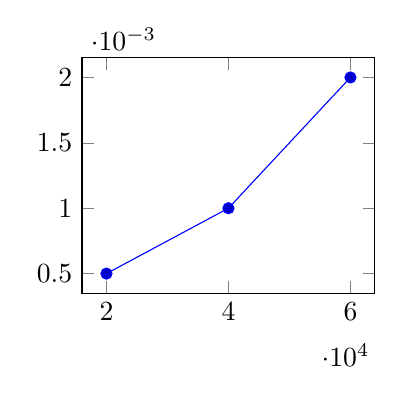
\begin{tikzpicture}
\begin{axis}[scaled ticks=true]
    \addplot coordinates {
        (20000,0.0005)
        (40000,0.0010)
        (60000,0.0020)
    };
\end{axis}
\end{tikzpicture}%
\end{codeexample}

\begin{codeexample}[]
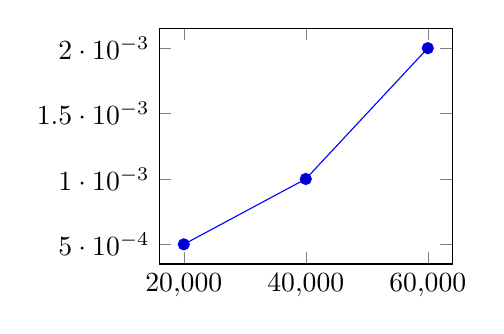
\begin{tikzpicture}
\begin{axis}[
    scaled ticks=false,
]
    \addplot coordinates {
        (20000,0.0005)
        (40000,0.0010)
        (60000,0.0020)
    };
\end{axis}
\end{tikzpicture}
\end{codeexample}

    键 |scaled ticks| 是一个样式，它简单地为 $x$ 和 $y$ 都设置刻度缩放。

    值 |base 10:|\meta{e} 允许手动调整算法。例如，|base 10:3| 会将每个刻度标签除以 $10^3$：
    %
\begin{codeexample}[]
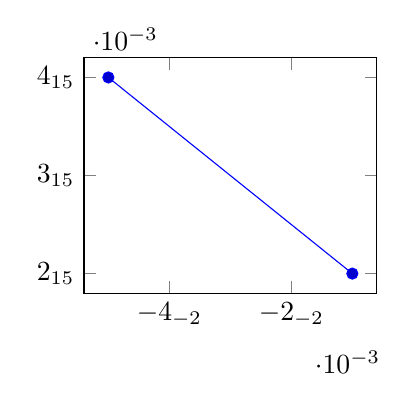
\begin{tikzpicture}
\begin{axis}[
    scaled ticks=base 10:3,
    /pgf/number format/sci subscript,
]
    \addplot coordinates {
        (-0.00001,2e12) (-0.00005,4e12)
    };
\end{axis}
\end{tikzpicture}
\end{codeexample}
    %
    \noindent 这里，\texttt{sci subscript} 选项只是为了节省空间。一般来说，|base 10:|$e$ 会将每个刻度除以 $10^e$。其效果不受上述“太大或太小”判断的限制。

    值 |real:|\meta{num} 允许将每个刻度除以固定的 \meta{num}。例如，下图的物理范围是 $0$ 到 $2\pi$，但刻度缩放算法被配置为将每个刻度标签除以 $\pi$。
    %
\begin{codeexample}[]
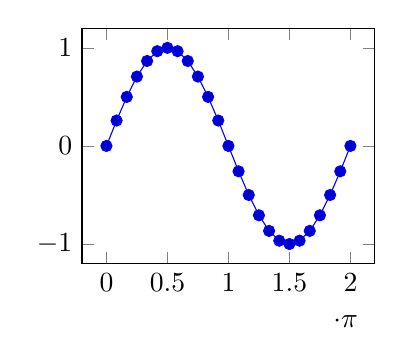
\begin{tikzpicture}
\begin{axis}[
    xtick={0,1.5708,...,10},
    domain=0:2*pi,
    scaled x ticks={real:3.1415},
    xtick scale label code/.code={$\cdot \pi$},
]
    \addplot {sin(deg(x))};
\end{axis}
\end{tikzpicture}
\end{codeexample}
    %
    \noindent 设置 |scaled ticks=real:|\meta{num} 还会将 |tick scale label code| 更改为
    %
\begin{codeexample}[code only]
\pgfkeys{/pgfplots/xtick scale label code/.code=
    {$\pgfkeysvalueof{/pgfplots/tick scale binop} \pgfmathprintnumber{#1}$},
}
\end{codeexample}
    %
    \noindent 键 |tick scale binop| 见下文，它初始设置为 |\cdot|。

    下面展示另一个——不太有用的——示例。每个 $x$ 刻度标签都除以 $2$，每个 $y$ 刻度标签都除以 $3$。
    %
\nobreak
\begin{codeexample}[]
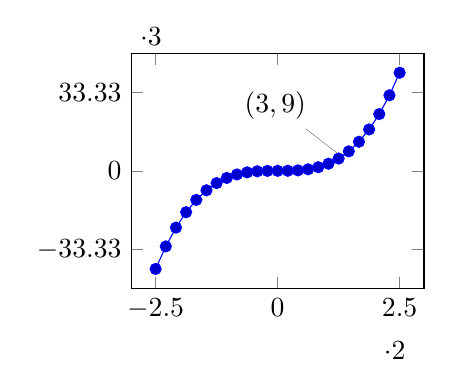
\begin{tikzpicture}
\begin{axis}[
    scaled x ticks=real:2,
    scaled y ticks=real:3,
]
    \addplot {x^3};
    \node [pin=135:{$(3,9)$}] at (3,9) {};
\end{axis}
\end{tikzpicture}
\end{codeexample}

    最后一个选项 |scaled ticks=manual:|\marg{label}\marg{code} 允许更多的自定义。它允许对显示的缩放标签\emph{以及}缩放代码进行\emph{完全控制}：\meta{label} 按其原样用于刻度缩放标签内部，而 \meta{code} 应该是一个带一个参数的宏，用于缩放每个刻度。示例：
    %
\begin{codeexample}[]
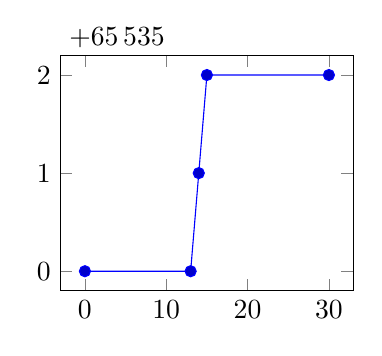
\begin{tikzpicture}
\begin{axis}[
    scaled y ticks=manual:{$+65\,535$}{
        \pgfmathparse{#1-65535}
    },
    yticklabel style={
        /pgf/number format/fixed,
        /pgf/number format/precision=1,
    },
]
    \addplot coordinates {
        (0, 65535)
        (13, 65535)
        (14, 65536)
        (15, 65537)
        (30, 65537)
    };
\end{axis}
\end{tikzpicture}
\end{codeexample}
    %
    \noindent 该示例使用 |$+65\,535$| 作为刻度缩放标签内容。此外，它定义了自定义刻度标签公式 $y - (+6.5535\cdot 10^4) = y - 65535$ 来生成 $y$ 刻度标签。

    \meta{label} 可以是任意的。它完全由用户控制。第二个参数 \meta{code} 应该是一个带一个参数的宏，其中 |#1| 是浮点表示形式的当前刻度位置。该宏应将结果赋值给 |\pgfmathresult|（作为数字）。\PGF{} 手册~\cite{tikz} 包含关于其数学引擎的详细文档。

    如果坐标无法用 \PGFPlots{} 处理，此功能也可用于变换坐标：变换它们并提供适当的刻度缩放方法，使刻度标签表示原始范围。

    如果 \meta{label} 为空，则不会绘制刻度缩放标签（也不占用空间）。

    刻度缩放\emph{不}适用于对数坐标轴。
\end{pgfplotsxykeylist}

\begin{pgfplotsxycodekeylist}{\x tick scale label code}
    允许更改缩放刻度标签的默认代码。默认为
    %
\begin{codeexample}[code only]
\pgfplotsset{
    xtick scale label code/.code={$\cdot 10^{#1}$},
}
\end{codeexample}

    更准确地说，它是
    %
\begin{codeexample}[code only]
\pgfplotsset{
    xtick scale label code/.code={$\pgfkeysvalueof{/pgfplots/tick scale binop} 10^{#1}$},
}
\end{codeexample}
    %
    \noindent 而 |tick scale binop| 的初始值是 |\cdot|，但如果需要可以更改为 |\times|。

    如果代码为空，则不会绘制刻度缩放标签（也不占用空间）。
\end{pgfplotsxycodekeylist}

\begin{pgfplotscodekey}{tick scale label code}
    一个样式，用于设置 |xtick scale label code| 以及 $y$ 和 $z$ 的对应项。
\end{pgfplotscodekey}

\begin{pgfplotskey}{tick scale binop=\marg{\TeX{} math operator} (initially \textbackslash cdot)}
    设置用于显示刻度缩放标签的二元运算符。
    %
\begin{codeexample}[]
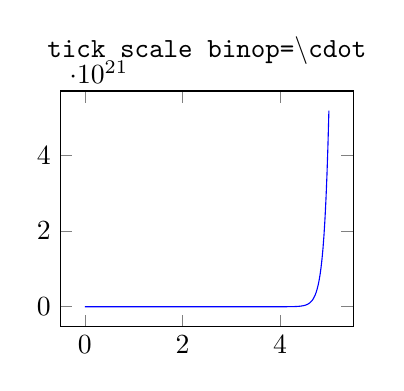
\begin{tikzpicture}
\begin{axis}[
    title=\texttt{tick scale
        binop=\textbackslash cdot},
]
    \addplot [
        mark=none,
        blue,
        samples=250,
        domain=0:5,
    ] {exp(10*x)};
\end{axis}
\end{tikzpicture}
\end{codeexample}

\begin{codeexample}[]
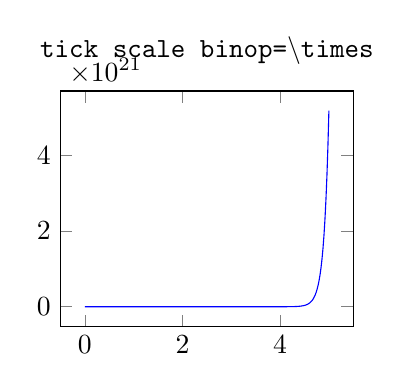
\begin{tikzpicture}
\begin{axis}[
    title=\texttt{tick scale
        binop=\textbackslash times},
    tick scale binop=\times,
]
    \addplot [
        mark=none,
        blue,
        samples=250,
        domain=0:5,
    ] {exp(10*x)};
\end{axis}
\end{tikzpicture}
\end{codeexample}
\end{pgfplotskey}

\makeatletter
    \let\itsinitial=\pgfplots@scale@ticks@below@exponent
\makeatother
\begin{pgfplotskey}{scale ticks below exponent=\marg{exponent} (initially \itsinitial)}
    允许微调 `|scaled ticks|' 算法：如果坐标轴界限的量级为 $10^e$ 且 $e<$\meta{exponent}，则公共前置因子~$10^e$ 将被提取出来。默认为
\end{pgfplotskey}

\makeatletter
    \let\itsinitial=\pgfplots@scale@ticks@above@exponent
\makeatother
\begin{pgfplotskey}{scale ticks above exponent=\marg{exponent} (initially \itsinitial)}
    允许微调 '|scaled ticks|' 算法：如果坐标轴界限的量级为 $10^e$ 且 $e>$\meta{exponent}，则公共前置因子~$10^e$ 将被提取出来。
\end{pgfplotskey}


\subsection{刻度微调}

刻度放置算法依赖于多个参数，可以调整这些参数以获得更好的结果。

\begin{pgfplotskey}{max space between ticks=\marg{number} (initially \axisdefaulttickwidth)}
\label{maxspacebetweenticks}
    以整磅为单位配置相邻刻度之间的最大间距。必须省略后缀 ``|pt|''，且不支持小数。
\end{pgfplotskey}

\begin{pgfplotskey}{try min ticks=\marg{number} (initially \axisdefaulttryminticks)}
    配置刻度数量的一个宽松下限。它应被视为建议，而非严格限制。如果 `|max space between ticks|' 产生的刻度太少，此数字会增加刻度数量。

    刻度总数仍可能变化，因为坐标轴范围内并非所有小数都是有效的刻度位置。
\end{pgfplotskey}

\begin{pgfplotskey}{try min ticks log=\marg{number} (initially 3)}
    与 |try min ticks| 相同，但用于对数坐标轴。
\end{pgfplotskey}

\begin{pgfplotskeylist}{%
    tickwidth=\marg{dimension} (initially 0.15cm),
    major tick length=\marg{dimension} (initially 0.15cm)%
}
    设置主刻度线的长度。

    可以使用 |\pgfkeysvalueof{/pgfplots/major tick length}| 访问它。
\end{pgfplotskeylist}

\begin{pgfplotskeylist}{%
    subtickwidth=\marg{dimension} (initially 0.1cm),
    minor tick length=\marg{dimension} (initially 0.1cm)%
}
    设置次刻度线的长度。

    可以使用 |\pgfkeysvalueof{/pgfplots/minor tick length}| 访问它。
\end{pgfplotskeylist}

\begin{pgfplotsxykeylist}{\x tick placement tolerance (initially 0.05pt)}
    如果刻度线和标签超出坐标轴界限不超过此容差，它们仍会被放置。选择此阈值时应使其不产生可见差异，同时仍提供容错能力。

    该阈值以最终图形的纸面单位给出。
\end{pgfplotsxykeylist}

\begin{pgfplotsxykey}{log basis \x=\marg{number} (initially empty)}
    允许更改用于对数坐标轴的对数。

    更改为不同的对数底数不过是一种缩放。然而，它也会改变刻度标签的显示方式：它们也将以新底数显示。
    %
\begin{codeexample}[]
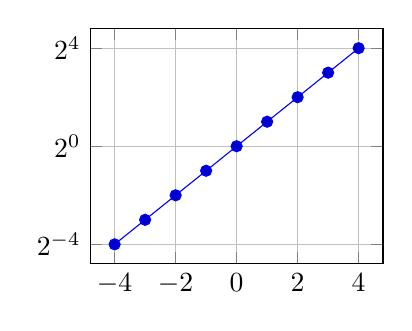
\begin{tikzpicture}
    \begin{semilogyaxis}[log basis y=2,grid=major,samples at={-4,...,4}]
        \addplot {2^x};
    \end{semilogyaxis}
\end{tikzpicture}
~
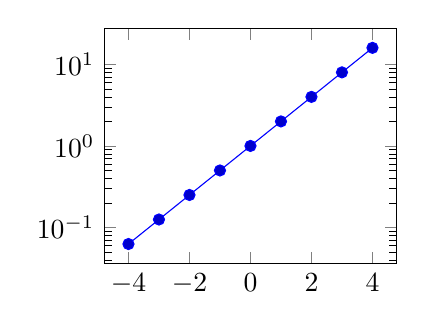
\begin{tikzpicture}
    \begin{semilogyaxis}[log basis y=10,samples at={-4,...,4}]
        \addplot {2^x};
    \end{semilogyaxis}
\end{tikzpicture}
\end{codeexample}

    初始设置为 `|log basis x=|'，其默认值为：对任何坐标使用自然对数（底数 $\exp(1)$），而刻度标签的显示使用对数底数 $10$。

    如果对数底数更改为非空字符串，则所选对数将应用于任何输入坐标（如果坐标轴缩放也是对数），并且刻度标签将以此底数显示。

    换句话说：通常，你看到的对数坐标轴底数就是 $10$，仅此而已。它仅对坐标过滤器有意义：初始设置（空 \meta{number}）对坐标列表使用底数 $e$，尽管显示将使用底数~$10$（即它被重新缩放）。任何非空值 \meta{number} 都会使坐标列表\emph{和}显示都使用 \meta{number} 作为对数的底数。|clickable| 库的 JavaScript 代码在计算斜率时将始终使用\emph{显示}底数（通常为 $10$）。


    \paragraph{技术说明。}

%    When |log basis x| is used, the style |log basis ticks=|\marg{axis char}
%    \todosp{this style is not documented so far, right?}
%    will be installed (in this case |log basis ticks=x|). This style in turn
%    will change |log number format code|.

    请注意，|xtickten| 现在的用法有所不同：它将以新底数提供所需的刻度！尽管名称 ``|ten|'' 有误导性，但如果设置了 |log basis x=2|，|xtickten={1,2,3,4}| 将在 $2^1,2^2,2^3,2^4$ 处产生刻度。
\end{pgfplotsxykey}

\begin{pgfplotsxykey}{hide obscured \x\space ticks=\mchoice{true,false} (initially true)}
    允许配置当 \PGFPlots{} 认为刻度及其标签被其他坐标轴线遮挡时是否应将其隐藏。
    %
\begin{codeexample}[]
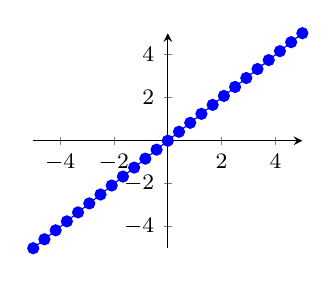
\begin{tikzpicture}
\begin{axis}[
    footnotesize,
    axis x line=center,
    axis y line=center,
    %hide obscured x ticks=false,
    %hide obscured y ticks=false,
]
    \addplot {x};
\end{axis}
\end{tikzpicture}
\end{codeexample}
\begin{codeexample}[]
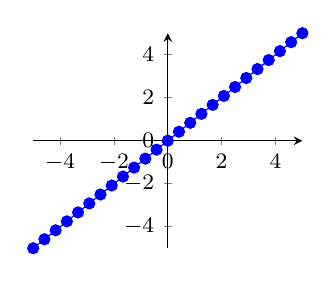
\begin{tikzpicture}
\begin{axis}[
    footnotesize,
    axis x line=center,
    axis y line=center,
    hide obscured x ticks=false,
    hide obscured y ticks=false,
]
    \addplot {x};
\end{axis}
\end{tikzpicture}
\end{codeexample}
    %
    请注意，此键仅当且仅当 |axis x line|、|axis y line| 或 |axis z line| 之一\emph{不}是 |box| 时才适用。
\end{pgfplotsxykey}
